\chapter{ROE MVA Control Plots}\label{sec:roe-control-plots}
\section{ROE Clean-up \texorpdfstring{$\pi^0$}{π0} Training}\label{sec:ROE_pi0}

\subsection{Variable Importance}

\begin{longtable}{c|l|c|l}
& Name & Alias & Importance \\
\toprule 
0 &\texttt{\footnotesize chiProb} & $v_{0}$ & $0.280$ \\ 
1 &\texttt{\footnotesize useCMSFrame(daughterAngleInBetween(0,1))} & $v_{1}$ & $0.203$ \\ 
2 &\texttt{\footnotesize daughter(0,useCMSFrame(p))} & $v_{2}$ & $0.073$ \\ 
3 &\texttt{\footnotesize InvM} & $v_{3}$ & $0.072$ \\ 
4 &\texttt{\footnotesize daughter(1,clusterHighestE)} & $v_{4}$ & $0.061$ \\ 
5 &\texttt{\footnotesize daughter(1,clusterTheta)} & $v_{5}$ & $0.049$ \\ 
6 &\texttt{\footnotesize daughter(1,p)} & $v_{6}$ & $0.047$ \\ 
7 &\texttt{\footnotesize daughter(0,clusterHighestE)} & $v_{7}$ & $0.029$ \\ 
8 &\texttt{\footnotesize daughter(0,clusterTheta)} & $v_{8}$ & $0.024$ \\ 
9 &\texttt{\footnotesize daughter(0,clusterE9E25)} & $v_{9}$ & $0.018$ \\ 
10 &\texttt{\footnotesize daughter(0,minC2HDist)} & $v_{10}$ & $0.018$ \\ 
11 &\texttt{\footnotesize daughter(1,minC2HDist)} & $v_{11}$ & $0.017$ \\ 
12 &\texttt{\footnotesize daughter(1,clusterE9E25)} & $v_{12}$ & $0.016$ \\ 
13 &\texttt{\footnotesize useRestFrame(daughterAngleInBetween(0,1))} & $v_{13}$ & $0.014$ \\ 
14 &\texttt{\footnotesize daughter(1,clusterNHits)} & $v_{14}$ & $0.013$ \\ 
15 &\texttt{\footnotesize daughter(0,clusterNHits)} & $v_{15}$ & $0.011$ \\ 
16 &\texttt{\footnotesize daughter(0,clusterErrorE)} & $v_{16}$ & $0.009$ \\ 
17 &\texttt{\footnotesize daughter(1,clusterErrorE)} & $v_{17}$ & $0.009$ \\ 
18 &\texttt{\footnotesize SigMBF} & $v_{18}$ & $0.007$ \\ 
19 &\texttt{\footnotesize useCMSFrame(p)} & $v_{19}$ & $0.006$ \\ 
20 &\texttt{\footnotesize daughter(0,p)} & $v_{20}$ & $0.005$ \\ 
21 &\texttt{\footnotesize SigM} & $v_{21}$ & $0.005$ \\ 
22 &\texttt{\footnotesize daughter(1,useCMSFrame(p))} & $v_{22}$ & $0.005$ \\ 
23 &\texttt{\footnotesize useLabFrame(daughterAngleInBetween(0,1))} & $v_{23}$ & $0.005$ \\ 
24 &\texttt{\footnotesize p} & $v_{24}$ & $0.003$ \\ 
\bottomrule
\captionsetup{width=0.8\linewidth}
\caption{Variable names, aliases and importance in the scope of $\pi^0$ MVA training for ROE clean-up.}
\end{longtable}

\subsection{Variable Distributions}

\begin{figure}[H]
\centering
\captionsetup{width=0.8\linewidth}
\subfigure{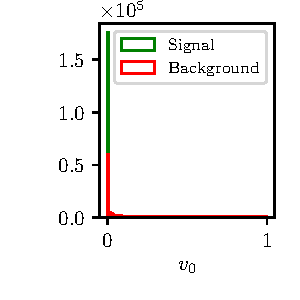
\includegraphics[width=0.241\linewidth]{fig/addendums/pi0_v0}}
\subfigure{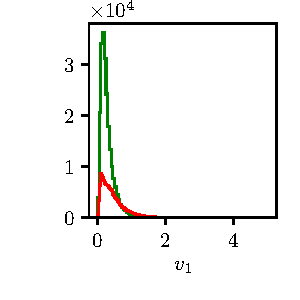
\includegraphics[width=0.241\linewidth]{fig/addendums/pi0_v1}}
\subfigure{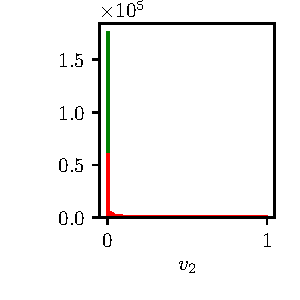
\includegraphics[width=0.241\linewidth]{fig/addendums/pi0_v2}}
\subfigure{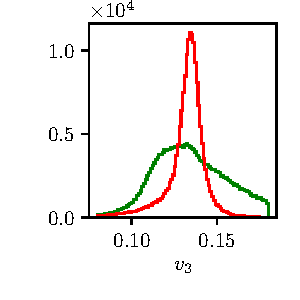
\includegraphics[width=0.241\linewidth]{fig/addendums/pi0_v3}}\\
\subfigure{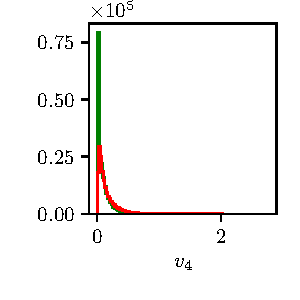
\includegraphics[width=0.241\linewidth]{fig/addendums/pi0_v4}}
\subfigure{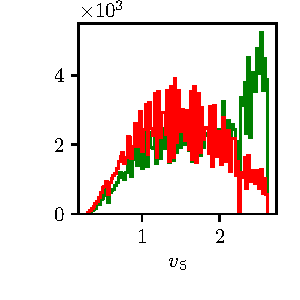
\includegraphics[width=0.241\linewidth]{fig/addendums/pi0_v5}}
\subfigure{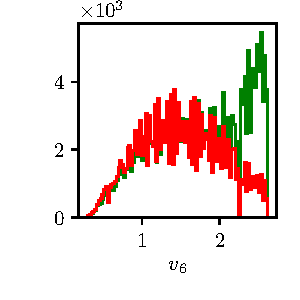
\includegraphics[width=0.241\linewidth]{fig/addendums/pi0_v6}}
\subfigure{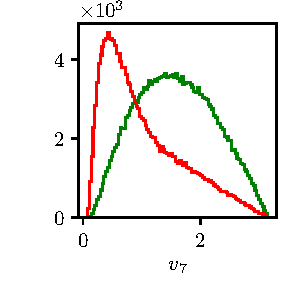
\includegraphics[width=0.241\linewidth]{fig/addendums/pi0_v7}}\\
\subfigure{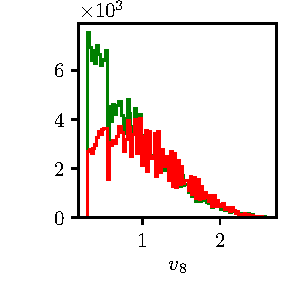
\includegraphics[width=0.241\linewidth]{fig/addendums/pi0_v8}}
\subfigure{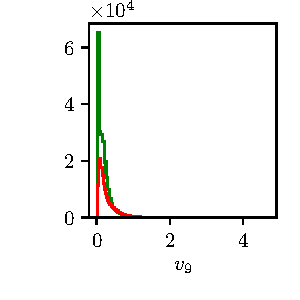
\includegraphics[width=0.241\linewidth]{fig/addendums/pi0_v9}}
\subfigure{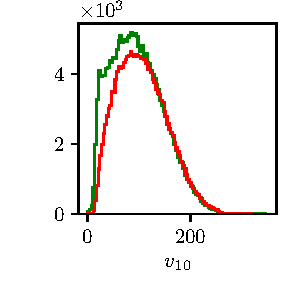
\includegraphics[width=0.241\linewidth]{fig/addendums/pi0_v10}}
\subfigure{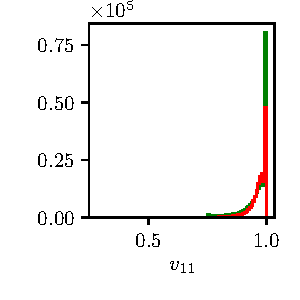
\includegraphics[width=0.241\linewidth]{fig/addendums/pi0_v11}}\\
\subfigure{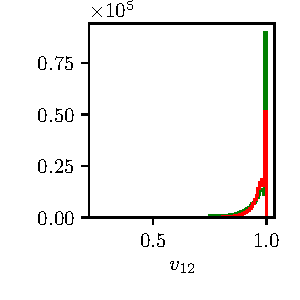
\includegraphics[width=0.241\linewidth]{fig/addendums/pi0_v12}}
\subfigure{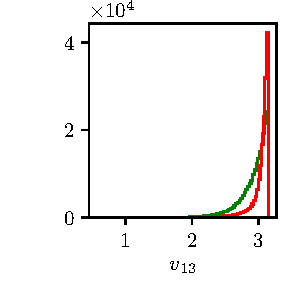
\includegraphics[width=0.241\linewidth]{fig/addendums/pi0_v13}}
\subfigure{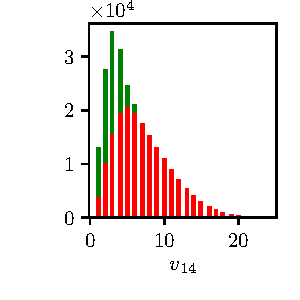
\includegraphics[width=0.241\linewidth]{fig/addendums/pi0_v14}}
\subfigure{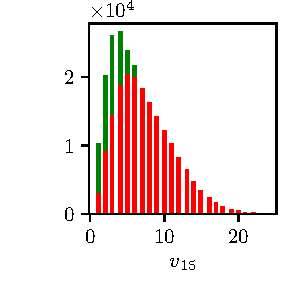
\includegraphics[width=0.241\linewidth]{fig/addendums/pi0_v15}}
\caption{Feature distributions for MVA training of $\pi^0$ candidates in the scope of ROE clean-up.}
\end{figure}

\begin{figure}[H]\ContinuedFloat
\captionsetup{width=0.8\linewidth}
\subfigure{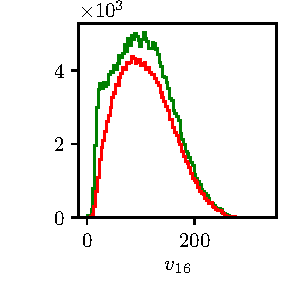
\includegraphics[width=0.241\linewidth]{fig/addendums/pi0_v16}}
\subfigure{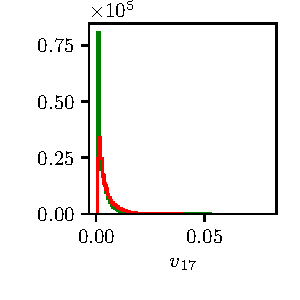
\includegraphics[width=0.241\linewidth]{fig/addendums/pi0_v17}}
\subfigure{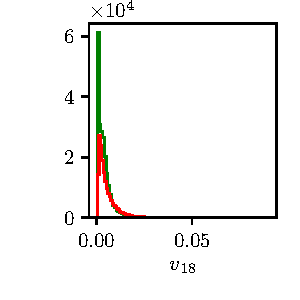
\includegraphics[width=0.241\linewidth]{fig/addendums/pi0_v18}}
\subfigure{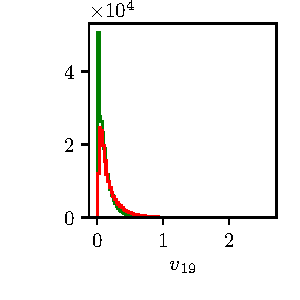
\includegraphics[width=0.241\linewidth]{fig/addendums/pi0_v19}}\\
\subfigure{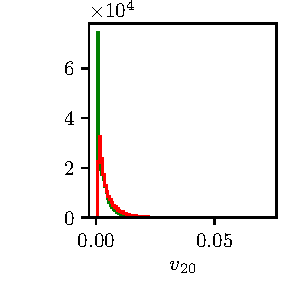
\includegraphics[width=0.241\linewidth]{fig/addendums/pi0_v20}}
\subfigure{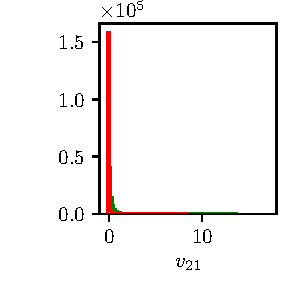
\includegraphics[width=0.241\linewidth]{fig/addendums/pi0_v21}}
\subfigure{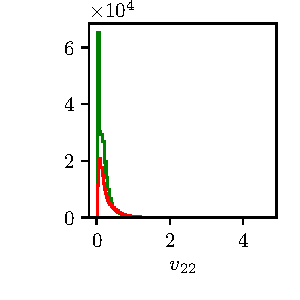
\includegraphics[width=0.241\linewidth]{fig/addendums/pi0_v22}}
\subfigure{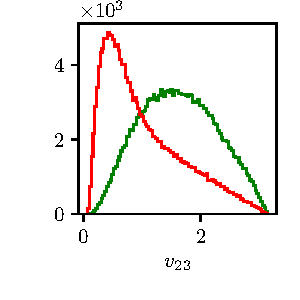
\includegraphics[width=0.241\linewidth]{fig/addendums/pi0_v23}}\\
\subfigure{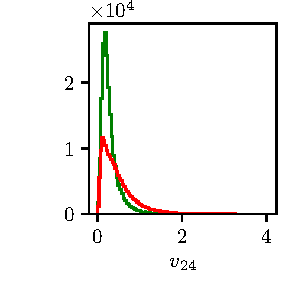
\includegraphics[width=0.241\linewidth]{fig/addendums/pi0_v24}}
\caption{Feature distributions for MVA training of $\pi^0$ candidates in the scope of ROE clean-up.}
\end{figure}

\subsection{Hyper-parameter Optimization}

\begin{figure}[H]
\centering
\captionsetup{width=0.8\linewidth}
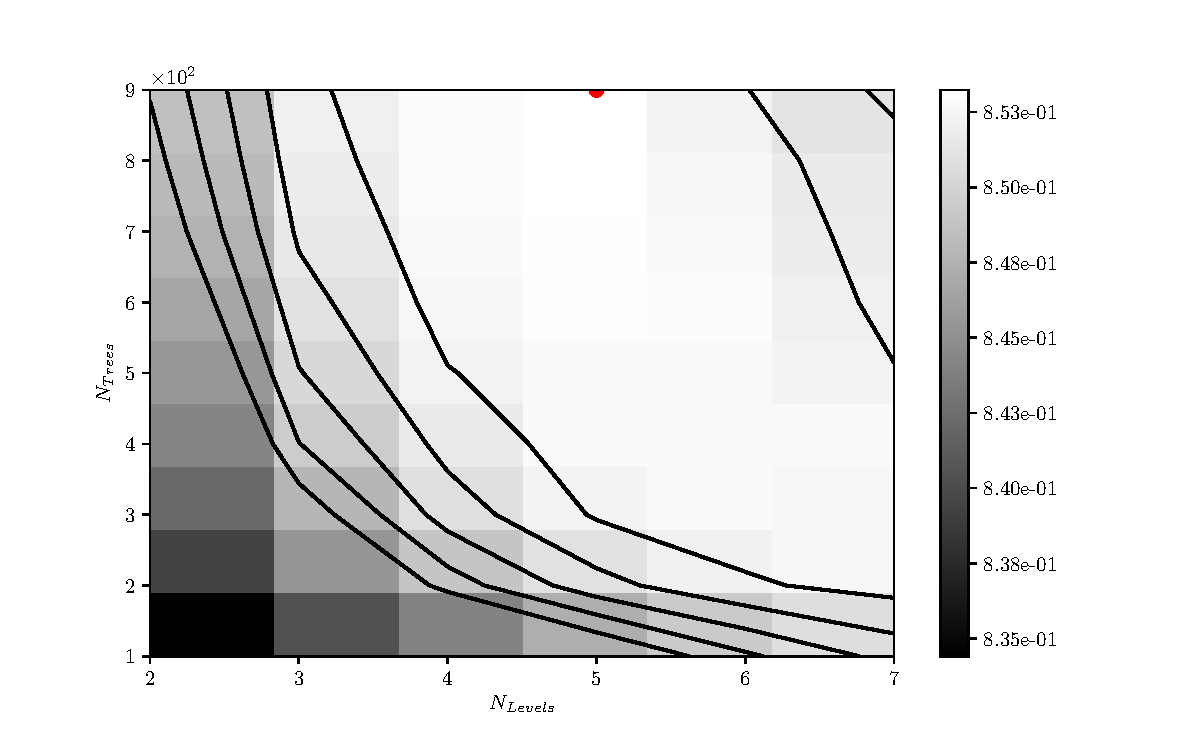
\includegraphics[width=\linewidth]{fig/addendums/pi0_hpo}
\caption{Hyper-parameter optimization of \texttt{\footnotesize nTrees} and \texttt{\footnotesize nLevels} in the BDT forest training of $\pi^0$ candidates in the scope of the ROE clean-up.}
\end{figure}

\subsection{Results}

\begin{figure}[H]
\centering
\captionsetup{width=0.8\linewidth}
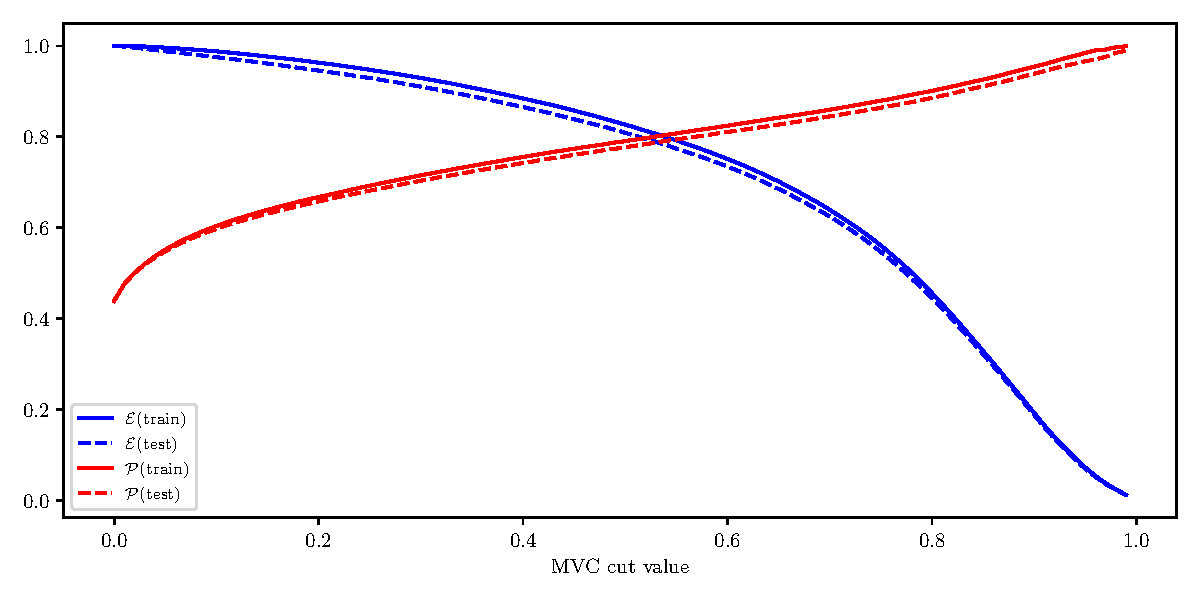
\includegraphics[width=\linewidth]{fig/addendums/pi0_effpur}
\caption{Efficiency ($\mathcal{E}$) and purity ($\mathcal{P}$) of the MVA classifier output for $\pi^0$ candidates training on the train (solid) and test (dashed) samples.}
\end{figure}

\begin{figure}[H]
\centering
\captionsetup{width=0.8\linewidth}
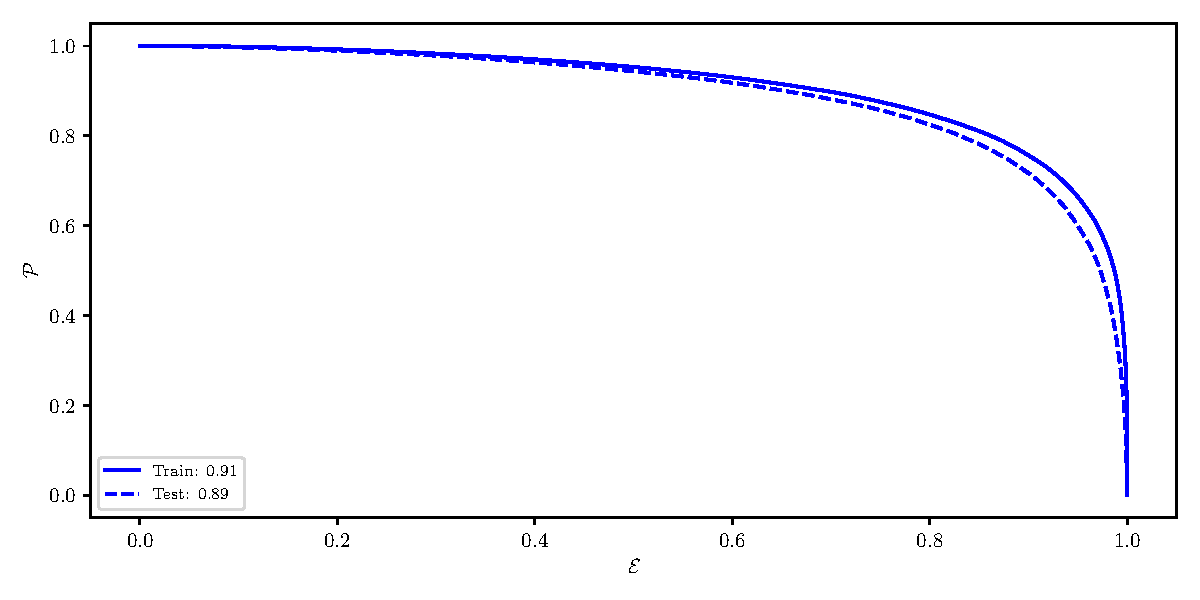
\includegraphics[width=\linewidth]{fig/addendums/pi0_roc}
\caption{ROC curves of the MVA classifier output for $\pi^0$ candidates training on the train (solid) and test (dashed) samples.}
\end{figure}

\section{ROE Clean-up \texorpdfstring{$\gamma$}{γ} Training}\label{sec:ROE_gamma}

\subsection{Variable Importance}

\begin{longtable}{c|l|c|l}
& Name & Alias & Importance \\
\toprule 
0 &\texttt{\footnotesize p} & $v_{0}$ & $0.327$ \\ 
1 &\texttt{\footnotesize pi0p} & $v_{1}$ & $0.243$ \\ 
2 &\texttt{\footnotesize clusterHighestE} & $v_{2}$ & $0.226$ \\ 
3 &\texttt{\footnotesize minC2HDist} & $v_{3}$ & $0.052$ \\ 
4 &\texttt{\footnotesize cosTheta} & $v_{4}$ & $0.036$ \\ 
5 &\texttt{\footnotesize clusterE9E25} & $v_{5}$ & $0.031$ \\ 
6 &\texttt{\footnotesize clusterNHits} & $v_{6}$ & $0.025$ \\ 
7 &\texttt{\footnotesize clusterUncorrE} & $v_{7}$ & $0.022$ \\ 
8 &\texttt{\footnotesize clusterR} & $v_{8}$ & $0.015$ \\ 
9 &\texttt{\footnotesize useCMSFrame(p)} & $v_{9}$ & $0.013$ \\ 
10 &\texttt{\footnotesize clusterErrorE} & $v_{10}$ & $0.010$ \\ 
11 &\texttt{\footnotesize clusterReg} & $v_{11}$ & $0.000$ \\ 
\bottomrule
\captionsetup{width=0.8\linewidth}
\caption{Variable names, aliases and importance in the scope of $\gamma$ MVA training for ROE clean-up.}
\end{longtable}


\subsection{Variable Distributions}

\begin{figure}[H]
\centering
\captionsetup{width=0.8\linewidth}
\subfigure{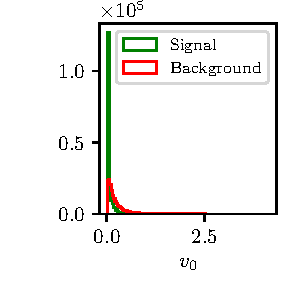
\includegraphics[width=0.241\linewidth]{fig/addendums/gamma_v0}}
\subfigure{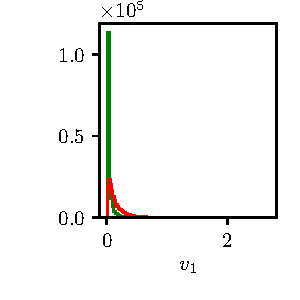
\includegraphics[width=0.241\linewidth]{fig/addendums/gamma_v1}}
\subfigure{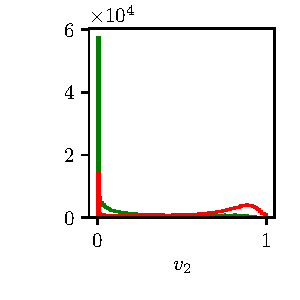
\includegraphics[width=0.241\linewidth]{fig/addendums/gamma_v2}}
\subfigure{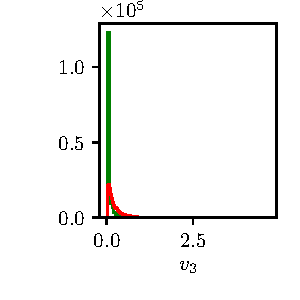
\includegraphics[width=0.241\linewidth]{fig/addendums/gamma_v3}}\\
\subfigure{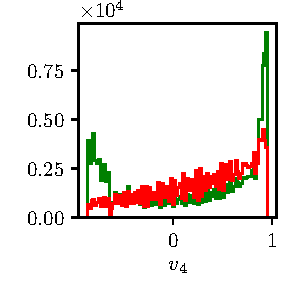
\includegraphics[width=0.241\linewidth]{fig/addendums/gamma_v4}}
\subfigure{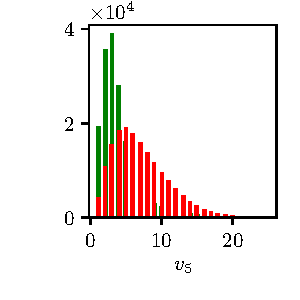
\includegraphics[width=0.241\linewidth]{fig/addendums/gamma_v5}}
\subfigure{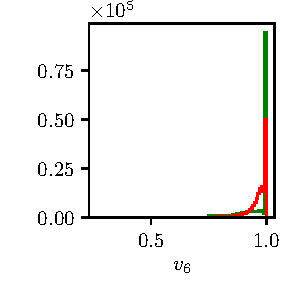
\includegraphics[width=0.241\linewidth]{fig/addendums/gamma_v6}}
\subfigure{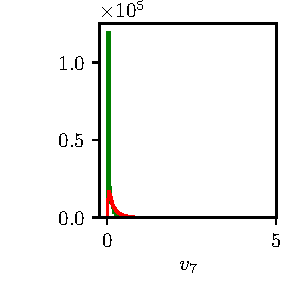
\includegraphics[width=0.241\linewidth]{fig/addendums/gamma_v7}}\\
\subfigure{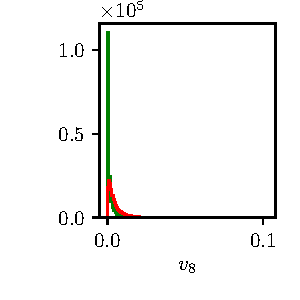
\includegraphics[width=0.241\linewidth]{fig/addendums/gamma_v8}}
\subfigure{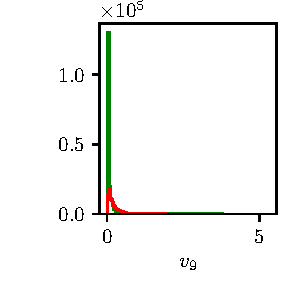
\includegraphics[width=0.241\linewidth]{fig/addendums/gamma_v9}}
\subfigure{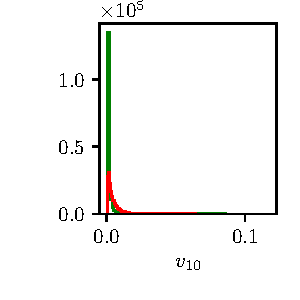
\includegraphics[width=0.241\linewidth]{fig/addendums/gamma_v10}}
\subfigure{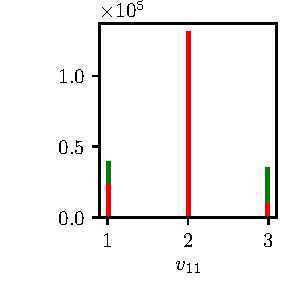
\includegraphics[width=0.241\linewidth]{fig/addendums/gamma_v11}}\\
\caption{Feature distributions for MVA training of $\gamma$ candidates in the scope of ROE clean-up.}
\end{figure}

\subsection{Hyper-parameter Optimization}

\begin{figure}[H]
\centering
\captionsetup{width=0.8\linewidth}
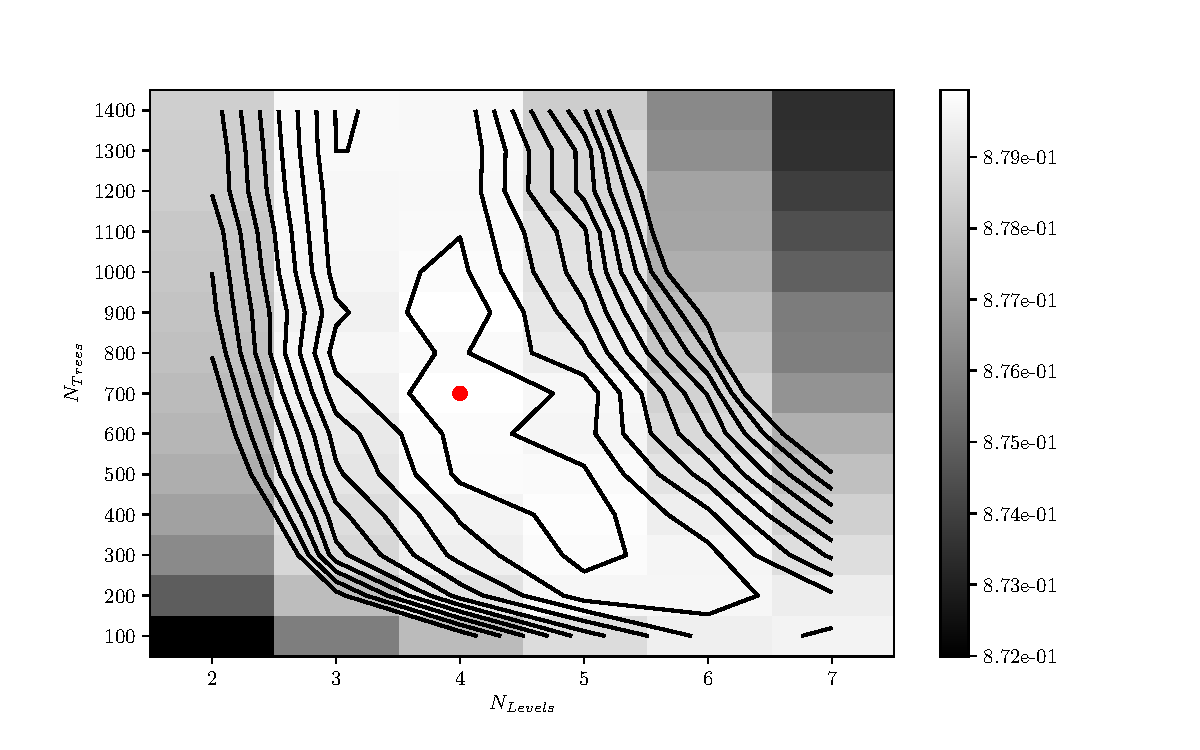
\includegraphics[width=\linewidth]{fig/addendums/gamma_hpo}
\caption{Hyper-parameter optimization of \texttt{\footnotesize nTrees} and \texttt{\footnotesize nLevels} in the BDT forest training of $\gamma$ candidates in the scope of the ROE clean-up.}
\end{figure}

\subsection{Results}

\begin{figure}[H]
\centering
\captionsetup{width=0.8\linewidth}
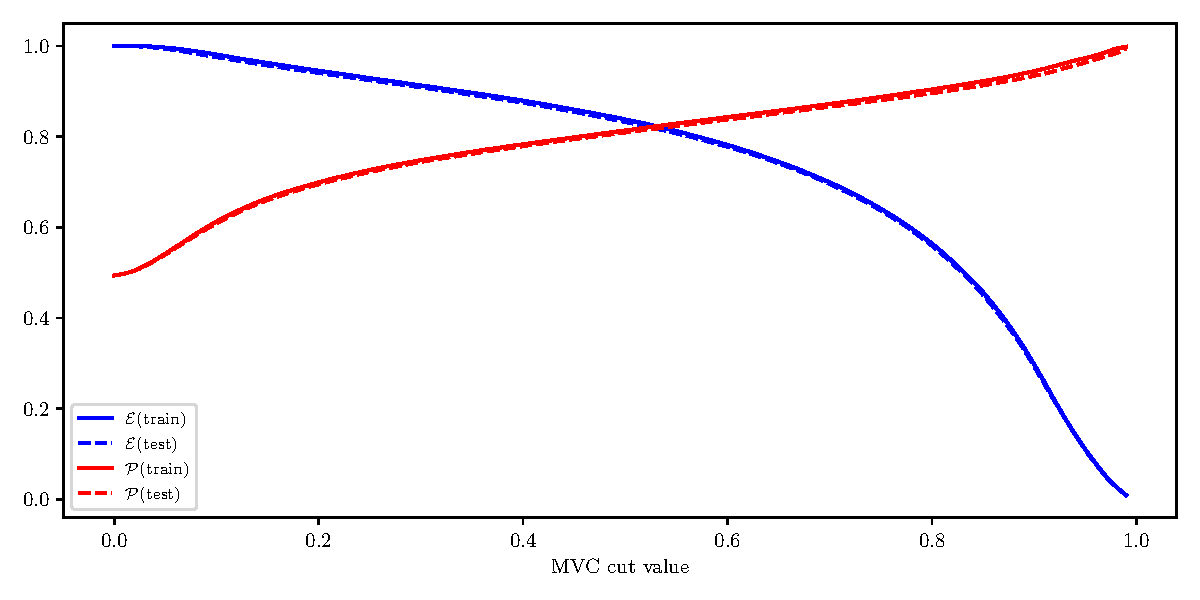
\includegraphics[width=\linewidth]{fig/addendums/gamma_effpur}
\caption{Efficiency ($\mathcal{E}$) and purity ($\mathcal{P}$) of the MVA classifier output for $\gamma$ candidates training on the train (solid) and test (dashed) samples.}
\end{figure}

\begin{figure}[H]
\centering
\captionsetup{width=0.8\linewidth}
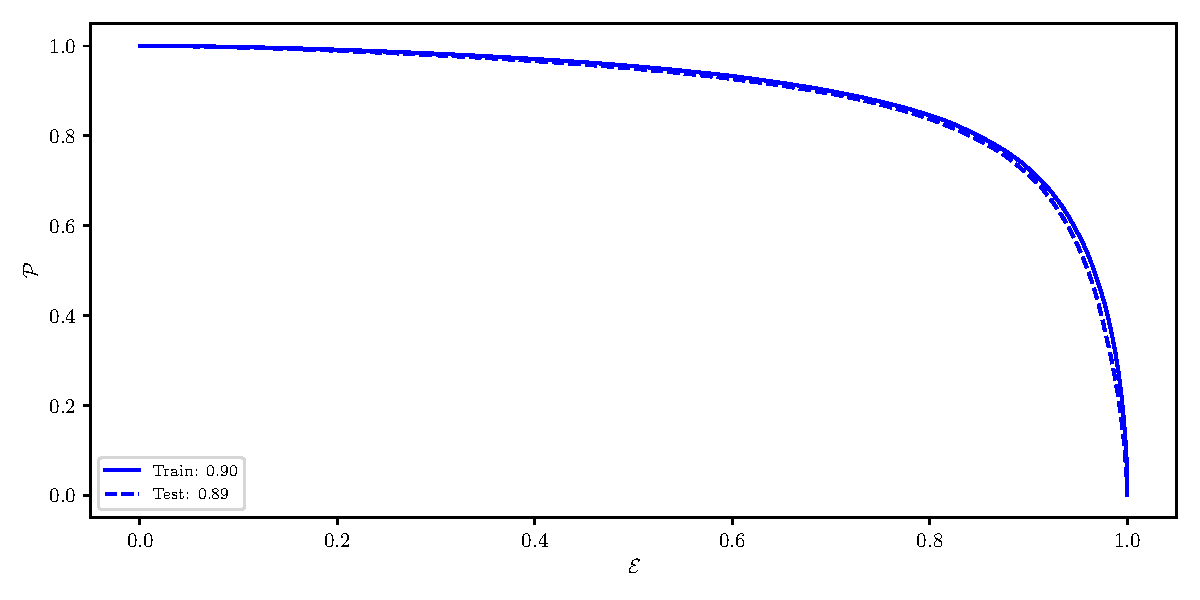
\includegraphics[width=\linewidth]{fig/addendums/gamma_roc}
\caption{ROC curves of the MVA classifier output for $\gamma$ candidates training on the train (solid) and test (dashed) samples.}
\end{figure}

\section{ROE Clean-up Duplicate Pair Training}\label{sec:ROE_dup}

\subsection{Variable Importance}

\begin{longtable}{c|l|c|l}
& Name & Alias & Importance \\
\toprule 
0 &\texttt{\footnotesize useCMSFrame(daughterAngleInBetween(0,1))} & $v_{0}$ & $0.132$ \\ 
1 &\texttt{\footnotesize daughter(0,phi0Err)} & $v_{1}$ & $0.082$ \\ 
2 &\texttt{\footnotesize useLabFrame(daughterAngleInBetween(0,1))} & $v_{2}$ & $0.055$ \\ 
3 &\texttt{\footnotesize daughter(1,d0)} & $v_{3}$ & $0.051$ \\ 
4 &\texttt{\footnotesize daughter(1,phi0Err)} & $v_{4}$ & $0.051$ \\ 
5 &\texttt{\footnotesize daughter(0,d0)} & $v_{5}$ & $0.050$ \\ 
6 &\texttt{\footnotesize daughter(1,nCDCHits)} & $v_{6}$ & $0.040$ \\ 
7 &\texttt{\footnotesize daughter(1,d0Err)} & $v_{7}$ & $0.037$ \\ 
8 &\texttt{\footnotesize daughter(0,nCDCHits)} & $v_{8}$ & $0.034$ \\ 
9 &\texttt{\footnotesize daughter(1,z0)} & $v_{9}$ & $0.032$ \\ 
10 &\texttt{\footnotesize daughter(0,z0)} & $v_{10}$ & $0.030$ \\ 
11 &\texttt{\footnotesize daughter(0,d0Err)} & $v_{11}$ & $0.028$ \\ 
12 &\texttt{\footnotesize daughter(0,nSVDHits)} & $v_{12}$ & $0.028$ \\ 
13 &\texttt{\footnotesize daughter(1,pz)} & $v_{13}$ & $0.027$ \\ 
14 &\texttt{\footnotesize daughter(1,useCMSFrame(p))} & $v_{14}$ & $0.024$ \\ 
15 &\texttt{\footnotesize extraInfo(decayModeID)} & $v_{15}$ & $0.023$ \\ 
16 &\texttt{\footnotesize daughter(0,pz)} & $v_{16}$ & $0.020$ \\ 
17 &\texttt{\footnotesize daughter(1,nSVDHits)} & $v_{17}$ & $0.020$ \\ 
18 &\texttt{\footnotesize daughter(0,pValue)} & $v_{18}$ & $0.020$ \\ 
19 &\texttt{\footnotesize daughter(1,tanlambda)} & $v_{19}$ & $0.018$ \\ 
20 &\texttt{\footnotesize daughter(1,pValue)} & $v_{20}$ & $0.018$ \\ 
21 &\texttt{\footnotesize daughter(0,tanlambda)} & $v_{21}$ & $0.017$ \\ 
22 &\texttt{\footnotesize daughter(0,phi0)} & $v_{22}$ & $0.016$ \\ 
23 &\texttt{\footnotesize daughter(1,phi0)} & $v_{23}$ & $0.016$ \\ 
24 &\texttt{\footnotesize daughter(0,useCMSFrame(p))} & $v_{24}$ & $0.015$ \\ 
25 &\texttt{\footnotesize daughter(0,z0Err)} & $v_{25}$ & $0.014$ \\ 
26 &\texttt{\footnotesize daughter(1,omega)} & $v_{26}$ & $0.013$ \\ 
27 &\texttt{\footnotesize daughter(0,omega)} & $v_{27}$ & $0.013$ \\ 
28 &\texttt{\footnotesize daughter(1,z0Err)} & $v_{28}$ & $0.012$ \\ 
29 &\texttt{\footnotesize daughter(0,pt)} & $v_{29}$ & $0.011$ \\ 
30 &\texttt{\footnotesize daughter(0,omegaErr)} & $v_{30}$ & $0.011$ \\ 
31 &\texttt{\footnotesize daughter(1,omegaErr)} & $v_{31}$ & $0.010$ \\ 
32 &\texttt{\footnotesize daughter(1,pt)} & $v_{32}$ & $0.009$ \\ 
33 &\texttt{\footnotesize daughter(0,tanlambdaErr)} & $v_{33}$ & $0.009$ \\ 
34 &\texttt{\footnotesize daughter(1,tanlambdaErr)} & $v_{34}$ & $0.009$ \\ 
35 &\texttt{\footnotesize useRestFrame(daughterAngleInBetween(0,1))} & $v_{35}$ & $0.003$ \\ 
36 &\texttt{\footnotesize daughter(1,charge)} & $v_{36}$ & $0.000$ \\ 
37 &\texttt{\footnotesize daughter(0,charge)} & $v_{37}$ & $0.000$ \\ 
\bottomrule
\captionsetup{width=0.8\linewidth}
\caption{Variable names, aliases and importance in the scope of duplicate track pair MVA training for ROE clean-up.}
\end{longtable}


\subsection{Variable Distributions}

\begin{figure}[H]
\centering
\captionsetup{width=0.8\linewidth}
\subfigure{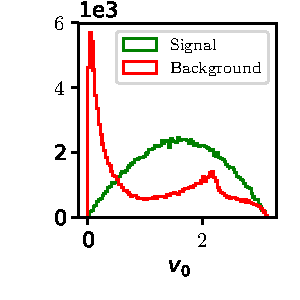
\includegraphics[width=0.241\linewidth]{fig/addendums/dup_v0}}
\subfigure{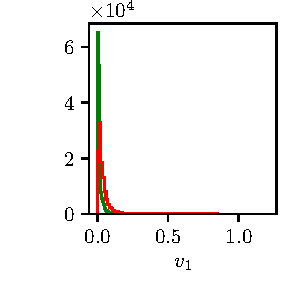
\includegraphics[width=0.241\linewidth]{fig/addendums/dup_v1}}
\subfigure{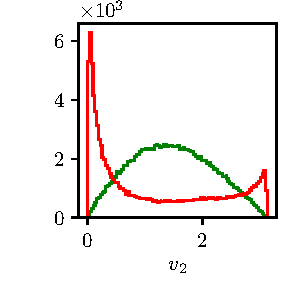
\includegraphics[width=0.241\linewidth]{fig/addendums/dup_v2}}
\subfigure{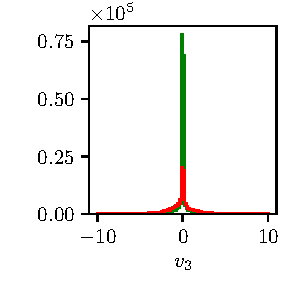
\includegraphics[width=0.241\linewidth]{fig/addendums/dup_v3}}\\
\subfigure{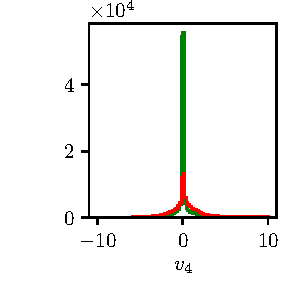
\includegraphics[width=0.241\linewidth]{fig/addendums/dup_v4}}
\subfigure{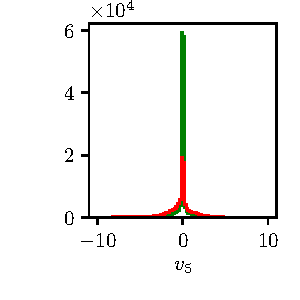
\includegraphics[width=0.241\linewidth]{fig/addendums/dup_v5}}
\subfigure{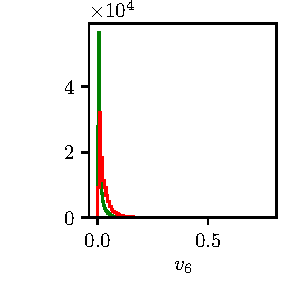
\includegraphics[width=0.241\linewidth]{fig/addendums/dup_v6}}
\subfigure{\includegraphics[width=0.241\linewidth]{fig/addendums/dup_v7}}\\
\subfigure{\includegraphics[width=0.241\linewidth]{fig/addendums/dup_v8}}
\subfigure{\includegraphics[width=0.241\linewidth]{fig/addendums/dup_v9}}
\subfigure{\includegraphics[width=0.241\linewidth]{fig/addendums/dup_v10}}
\subfigure{\includegraphics[width=0.241\linewidth]{fig/addendums/dup_v11}}\\
\subfigure{\includegraphics[width=0.241\linewidth]{fig/addendums/dup_v12}}
\subfigure{\includegraphics[width=0.241\linewidth]{fig/addendums/dup_v13}}
\subfigure{\includegraphics[width=0.241\linewidth]{fig/addendums/dup_v14}}
\subfigure{\includegraphics[width=0.241\linewidth]{fig/addendums/dup_v15}}\\
\subfigure{\includegraphics[width=0.241\linewidth]{fig/addendums/dup_v16}}
\subfigure{\includegraphics[width=0.241\linewidth]{fig/addendums/dup_v17}}
\subfigure{\includegraphics[width=0.241\linewidth]{fig/addendums/dup_v18}}
\subfigure{\includegraphics[width=0.241\linewidth]{fig/addendums/dup_v19}}
\caption{Feature distributions for MVA training of duplicate track pair candidates in the scope of ROE clean-up.}
\end{figure}

\begin{figure}[H]\ContinuedFloat
\captionsetup{width=0.8\linewidth}
\subfigure{\includegraphics[width=0.241\linewidth]{fig/addendums/dup_v20}}
\subfigure{\includegraphics[width=0.241\linewidth]{fig/addendums/dup_v21}}
\subfigure{\includegraphics[width=0.241\linewidth]{fig/addendums/dup_v22}}
\subfigure{\includegraphics[width=0.241\linewidth]{fig/addendums/dup_v23}}\\
\subfigure{\includegraphics[width=0.241\linewidth]{fig/addendums/dup_v24}}
\subfigure{\includegraphics[width=0.241\linewidth]{fig/addendums/dup_v25}}
\subfigure{\includegraphics[width=0.241\linewidth]{fig/addendums/dup_v26}}
\subfigure{\includegraphics[width=0.241\linewidth]{fig/addendums/dup_v27}}\\
\subfigure{\includegraphics[width=0.241\linewidth]{fig/addendums/dup_v28}}
\subfigure{\includegraphics[width=0.241\linewidth]{fig/addendums/dup_v29}}
\subfigure{\includegraphics[width=0.241\linewidth]{fig/addendums/dup_v30}}
\subfigure{\includegraphics[width=0.241\linewidth]{fig/addendums/dup_v31}}\\
\subfigure{\includegraphics[width=0.241\linewidth]{fig/addendums/dup_v32}}
\subfigure{\includegraphics[width=0.241\linewidth]{fig/addendums/dup_v33}}
\subfigure{\includegraphics[width=0.241\linewidth]{fig/addendums/dup_v34}}
\subfigure{\includegraphics[width=0.241\linewidth]{fig/addendums/dup_v35}}\\
\subfigure{\includegraphics[width=0.241\linewidth]{fig/addendums/dup_v36}}
\subfigure{\includegraphics[width=0.241\linewidth]{fig/addendums/dup_v37}}
\caption{Feature distributions for MVA training of duplicate track pair candidates in the scope of ROE clean-up.}
\end{figure}

\subsection{Hyper-parameter Optimization}

\begin{figure}[H]
\centering
\captionsetup{width=0.8\linewidth}
\includegraphics[width=\linewidth]{fig/addendums/dup_hpo}
\caption{Hyper-parameter optimization of \texttt{\footnotesize nTrees} and \texttt{\footnotesize nLevels} in the BDT forest training of duplicate track pair candidates in the scope of the ROE clean-up.}
\end{figure}

\subsection{Results}

\begin{figure}[H]
\centering
\captionsetup{width=0.8\linewidth}
\includegraphics[width=\linewidth]{fig/addendums/dup_effpur}
\caption{Efficiency ($\mathcal{E}$) and purity ($\mathcal{P}$) of the MVA classifier output for duplicate track pair candidates training on the train (solid) and test (dashed) samples.}
\end{figure}

\begin{figure}[H]
\centering
\captionsetup{width=0.8\linewidth}
\includegraphics[width=\linewidth]{fig/addendums/dup_roc}
\caption{ROC curves of the MVA classifier output for duplicate track pair candidates training on the train (solid) and test (dashed) samples.}
\end{figure}

\section{ROE Clean-up Duplicate Track Training}\label{sec:ROE_curl}

\subsection{Variable Importance}

\begin{longtable}{c|l|c|l}
& Name & Alias & Importance \\
\toprule 
0 &\texttt{\footnotesize extraInfo(d0Diff)} & $v_{0}$ & $0.214$ \\ 
1 &\texttt{\footnotesize extraInfo(z0Diff)} & $v_{1}$ & $0.087$ \\ 
2 &\texttt{\footnotesize d0} & $v_{2}$ & $0.069$ \\ 
3 &\texttt{\footnotesize extraInfo(pValueDiff)} & $v_{3}$ & $0.060$ \\ 
4 &\texttt{\footnotesize z0} & $v_{4}$ & $0.058$ \\ 
5 &\texttt{\footnotesize phi0Err} & $v_{5}$ & $0.056$ \\ 
6 &\texttt{\footnotesize extraInfo(pzDiff)} & $v_{6}$ & $0.055$ \\ 
7 &\texttt{\footnotesize extraInfo(ptDiff)} & $v_{7}$ & $0.045$ \\ 
8 &\texttt{\footnotesize z0Err} & $v_{8}$ & $0.043$ \\ 
9 &\texttt{\footnotesize extraInfo(nCDCHitsDiff)} & $v_{9}$ & $0.037$ \\ 
10 &\texttt{\footnotesize extraInfo(nSVDHitsDiff)} & $v_{10}$ & $0.034$ \\ 
11 &\texttt{\footnotesize pt} & $v_{11}$ & $0.032$ \\ 
12 &\texttt{\footnotesize d0Err} & $v_{12}$ & $0.030$ \\ 
13 &\texttt{\footnotesize pValue} & $v_{13}$ & $0.029$ \\ 
14 &\texttt{\footnotesize nCDCHits} & $v_{14}$ & $0.028$ \\ 
15 &\texttt{\footnotesize nSVDHits} & $v_{15}$ & $0.028$ \\ 
16 &\texttt{\footnotesize pz} & $v_{16}$ & $0.025$ \\ 
17 &\texttt{\footnotesize cosTheta} & $v_{17}$ & $0.024$ \\ 
18 &\texttt{\footnotesize phi0} & $v_{18}$ & $0.023$ \\ 
19 &\texttt{\footnotesize useCMSFrame(p)} & $v_{19}$ & $0.021$ \\ 
\bottomrule
\captionsetup{width=0.8\linewidth}
\caption{Variable names, aliases and importance in the scope of duplicate track MVA training for ROE clean-up.}
\end{longtable}


\subsection{Variable Distributions}

\begin{figure}[H]
\centering
\captionsetup{width=0.8\linewidth}
\subfigure{\includegraphics[width=0.241\linewidth]{fig/addendums/curl_v0}}
\subfigure{\includegraphics[width=0.241\linewidth]{fig/addendums/curl_v1}}
\subfigure{\includegraphics[width=0.241\linewidth]{fig/addendums/curl_v2}}
\subfigure{\includegraphics[width=0.241\linewidth]{fig/addendums/curl_v3}}\\
\subfigure{\includegraphics[width=0.241\linewidth]{fig/addendums/curl_v4}}
\subfigure{\includegraphics[width=0.241\linewidth]{fig/addendums/curl_v5}}
\subfigure{\includegraphics[width=0.241\linewidth]{fig/addendums/curl_v6}}
\subfigure{\includegraphics[width=0.241\linewidth]{fig/addendums/curl_v7}}\\
\subfigure{\includegraphics[width=0.241\linewidth]{fig/addendums/curl_v8}}
\subfigure{\includegraphics[width=0.241\linewidth]{fig/addendums/curl_v9}}
\subfigure{\includegraphics[width=0.241\linewidth]{fig/addendums/curl_v10}}
\subfigure{\includegraphics[width=0.241\linewidth]{fig/addendums/curl_v11}}\\
\subfigure{\includegraphics[width=0.241\linewidth]{fig/addendums/curl_v12}}
\subfigure{\includegraphics[width=0.241\linewidth]{fig/addendums/curl_v13}}
\subfigure{\includegraphics[width=0.241\linewidth]{fig/addendums/curl_v14}}
\subfigure{\includegraphics[width=0.241\linewidth]{fig/addendums/curl_v15}}\\
\subfigure{\includegraphics[width=0.241\linewidth]{fig/addendums/curl_v16}}
\subfigure{\includegraphics[width=0.241\linewidth]{fig/addendums/curl_v17}}
\subfigure{\includegraphics[width=0.241\linewidth]{fig/addendums/curl_v18}}
\subfigure{\includegraphics[width=0.241\linewidth]{fig/addendums/curl_v19}}
\caption{Feature distributions for MVA training of duplicate track candidates in the scope of ROE clean-up.}
\end{figure}

%\begin{figure}[H]\ContinuedFloat
%\captionsetup{width=0.8\linewidth}
%\subfigure{\includegraphics[width=0.241\linewidth]{fig/addendums/curl_v20}}
%\subfigure{\includegraphics[width=0.241\linewidth]{fig/addendums/curl_v21}}
%\subfigure{\includegraphics[width=0.241\linewidth]{fig/addendums/curl_v22}}
%\subfigure{\includegraphics[width=0.241\linewidth]{fig/addendums/curl_v23}}\\
%\subfigure{\includegraphics[width=0.241\linewidth]{fig/addendums/curl_v24}}
%\caption{Feature distributions for MVA training of duplicate track candidates in the scope of ROE clean-up.}
%\end{figure}

\subsection{Hyper-parameter Optimization}

\begin{figure}[H]
\centering
\captionsetup{width=0.8\linewidth}
\includegraphics[width=\linewidth]{fig/addendums/curl_hpo}
\caption{Hyper-parameter optimization of \texttt{\footnotesize nTrees} and \texttt{\footnotesize nLevels} in the BDT forest training of duplicate track candidates in the scope of the ROE clean-up.}
\end{figure}

\subsection{Results}

\begin{figure}[H]
\centering
\captionsetup{width=0.8\linewidth}
\includegraphics[width=\linewidth]{fig/addendums/curl_effpur}
\caption{Efficiency ($\mathcal{E}$) and purity ($\mathcal{P}$) of the MVA classifier output for duplicate track candidates training on the train (solid) and test (dashed) samples.}
\end{figure}

\begin{figure}[H]
\centering
\captionsetup{width=0.8\linewidth}
\includegraphics[width=\linewidth]{fig/addendums/curl_roc}
\caption{ROC curves of the MVA classifier output for duplicate track candidates training on the train (solid) and test (dashed) samples.}
\end{figure}